\documentclass[a4paper,12pt]{article}
\usepackage[T1]{fontenc}
\usepackage{parskip} % Removes paragraph indentation, adds vertical space between paragraphs
\usepackage{
    abraces, algorithm, algpseudocode, amsfonts, amsmath, amssymb, amsthm, bm, enumitem, graphicx, mathtools, subcaption
}
\usepackage{natbib}
\usepackage{newtxtext,newtxmath} % modern, Times-like + proper math. Or \usepackage{lmodern}
\usepackage{zi4} % provides the Inconsolata monospaced font, but in a LaTeX-ready form
\usepackage[raggedright]{titlesec} % in case for long titles
\usepackage[breaklinks]{hyperref} % allow breaklines for references
\usepackage{cleveref} % load after hyperref package
\usepackage[a4paper,left=3cm,right=3cm,top=3cm,bottom=3cm]{geometry}
\raggedbottom % don't force equal height pages. Or \flushbottom to make make pages equal height
\allowdisplaybreaks % allow page breaks inside equations 
\graphicspath{{./imgs/}{../benchmark/}{../figs/}}

\newtheorem{theorem}{Theorem}[section]
\newtheorem{definition}{Definition}[section]
\newtheorem{remark}{Remark}[section]
\newtheorem{lemma}{Lemma}[section]
\newtheorem{corollary}{Corollary}[section]
\newtheorem{prop}{Proposition}[section]

\DeclareMathOperator{\Arg}{Arg} % Branch argument of complex numbers
\DeclareMathOperator{\Var}{Var} % variance
\DeclareMathOperator{\Cov}{Cov} % covariance
\DeclareMathOperator{\corr}{corr} % correlation
\DeclareMathOperator{\Int}{Int} % interior
\DeclareMathOperator{\Ext}{Ext} % exterior
\DeclareMathOperator{\Res}{Res} % residule
\DeclareMathOperator{\tr}{tr} % trace
\DeclareMathOperator*{\argmax}{arg\,max} % argmax
\DeclareMathOperator*{\argmin}{arg\,min} % argmin
\DeclarePairedDelimiter\abs{\lvert}{\rvert} % absolute value
\DeclarePairedDelimiter\norm{\lVert}{\rVert} % norm

% Swap the definition of \abs* and \norm*, so that \abs
% and \norm resizes the size of the brackets, and the
% starred version does not.
\makeatletter
\let\oldabs\abs
\def\abs{\@ifstar{\oldabs}{\oldabs*}}
%
\let\oldnorm\norm
\def\norm{\@ifstar{\oldnorm}{\oldnorm*}}


\begin{document}
\pagenumbering{gobble} % Turn off page numbering until first section.

% Title page
\begin{titlepage}
\begin{center}
\vspace{1cm}
\textsf{\Huge{University of Oxford \\}}
\vspace{1cm}
\begin{figure}[htb]
\centering

\includegraphics[scale=.8]{stats_logo_RGB.jpg}
\end{figure}
\vspace{2.0cm}
\Huge{Score-Based Diffusion Models for Protein Backbone Generation\\}
\vspace{2.0cm}
\large{ by \\[14pt] Yuanhao Jiang \\[8pt] Wolfson College} \\
\vspace{2.2cm}
\large{A dissertation submitted in partial fulfilment of the degree of Master of Science in Statistical Science.
} \\
\vspace{.5cm}
\large{\emph{Department of Statistics, 24--29 St Giles, \\Oxford, OX1 3LB}} \\
\vspace{1.0cm}
\large{September 2025} \\
\end{center}
\end{titlepage}
\clearpage

This is my own work (except where otherwise indicated)
\vspace{2.5in}

\begin{center}
Candidate: Yuanhao Jiang\\
\vspace{1.0in}
Signed:.................................\\
\vspace{1.0in}
Date:...................................
\end{center}
\clearpage
\begin{abstract}

The abstract should go here.

\end{abstract}
\clearpage
\vspace*{2in}
\begin{center}
\textbf{Acknowledgements}
\end{center}

I would like to thank the following:
\clearpage

\tableofcontents
\listoffigures
\listoftables
\clearpage

\pagenumbering{arabic}

\section{Introduction}
\subsection{Background on Diffusion Models}
Diffusion models have recently emerged as one of the most powerful classes of deep generative models, achieving state-of-the-art performance in a wide range of domains, most prominently in image generation \cite{hoDenoisingDiffusionProbabilistic2020, dhariwal2021DiffusionModelsBeat}. These models construct a forward process that gradually corrupts data with Gaussian noise and train a neural network to approximate the reverse-time dynamics that iteratively remove noise. The resulting generative process is both probabilistically principled and empirically effective, offering advantages in sample quality and training stability compared to earlier paradigms such as variational autoencoders (VAEs) \cite{kingma2022AutoEncodingVariationalBayes} and generative adversarial networks (GANs) \cite{goodfellow2020GenerativeAdversarialNetworks}.

Score-based diffusion models \cite{song2021ScoreBasedGenerativeModeling,songMaximumLikelihoodTraining2021} improve discrete-time denoising diffusion probabilistic models with continuous-time stochastic differential equations (SDEs). Instead of directly parameterising the reverse process, they learn the score function---the gradient of the log-density of the noisy distribution---which enables the use of a variety of forward SDEs and corresponding reverse-time samplers. This framework has proven highly flexible and has been successfully applied to domains including image generation, audio synthesis, point clouds, and molecular data.

\subsection{Motivation: Protein Structure Generation}
Proteins are essential macromolecules whose biological functions are determined by their three-dimensional structures. The ability to generate novel protein structures has immense implications for biomedical science, including de novo protein design, drug discovery, and enzyme engineering. However, protein structures are highly constrained: bond lengths and angles must remain within narrow physical ranges, torsional angles follow characteristic distributions, and valid folds must satisfy global topological requirements. These constraints make the generative task significantly more challenging than in image or text domains.

Recent advances in deep learning, most notably AlphaFold \cite{jumper2021HighlyAccurateProtein}, have demonstrated the power of data-driven models in predicting native structures from sequence. Yet, the problem of generating realistic, diverse backbones without explicit sequence conditioning remains an open challenge.

\subsection{Diffusion Models for Protein Structures}
The probabilistic formulation of score-based diffusion models makes them a natural candidate for modelling protein structures. Unlike GANs, diffusion models provide a likelihood-based framework, and unlike VAEs, they avoid restrictive parametric assumptions about the latent space. Moreover, their iterative denoising dynamics align well with the notion of refining approximate structures toward physically plausible conformations.

Recent work has demonstrated the potential of diffusion-based approaches in protein modelling and design. For example, RFdiffusion \cite{watsonNovoDesignProtein2023} introduced a powerful framework for de novo protein design, achieving unprecedented results in generating novel folds and functional structures. FoldingDiff \cite{wuProteinStructureGeneration2024} proposed a diffusion-based model that explicitly learns the folding process, while DiffDock \cite{yimDiffusionModelsProtein2024} applied diffusion models to protein-ligand docking, highlighting the versatility of the paradigm in structural biology. These developments underscore the promise of diffusion generative models in capturing the rich geometric and biophysical constraints inherent to protein structures.

Applying diffusion models to proteins requires careful representation choices. 
In this work, we consider the protein backbone as a graph where nodes correspond to C\(\alpha\) atoms and edges encode both spatial proximity and sequential adjacency. 
This enables the use of graph neural networks (GNNs) \cite{scarselliGraphNeuralNetwork2009} as score models, incorporating geometric information through radial basis encodings, directional vectors, and positional embeddings. 
By training such models on large structural datasets, it becomes possible to learn score functions over protein conformational space and to generate new backbone structures through reverse diffusion.

\subsection{Structure of the Dissertation}
\Cref{sec:SBD} presents the theoretical foundations of score-based diffusion, the representation of protein backbones, and the model architectures explored. \Cref{sec:Experiments} describes the experimental setup, training procedure, and evaluation metrics, and reports quantitative and qualitative results. And discusses the implications of our findings, limitations, and avenues for future research. \Cref{sec:Discussion_and_Conclusion} concludes the dissertation by summarising contributions and highlighting potential future directions.

\clearpage

\section{Score-Based Diffusion for Generative Modelling}\label{sec:SBD}
\subsection{Background and Motivation}
Generative modelling aims to learn a distribution from which new samples can be drawn that resemble those observed in a dataset. Classical approaches include variational autoencoders (VAEs)~\citep{kingma2022AutoEncodingVariationalBayes}, which maximise a variational lower bound on the likelihood, and generative adversarial networks (GANs)~\citep{goodfellow2020GenerativeAdversarialNetworks}, which frame generation as an adversarial game. While each of these paradigms has been successful, they also suffer from characteristic drawbacks such as blurry reconstructions (VAEs) and mode collapse (GANs).

Diffusion models represent a more recent class of generative models that address many of these limitations. The central idea is deceptively simple: one defines a forward process that gradually corrupts data with noise until the signal is destroyed, and then learns a reverse process that reconstructs data from noise. By formulating the forward process as a diffusion and training a neural network to approximate the reverse dynamics, diffusion models combine the flexibility of deep networks with the probabilistic rigour of latent-variable models. 

In their original formulation, denoising diffusion probabilistic models (DDPMs)~\citep{hoDenoisingDiffusionProbabilistic2020} defined the forward process as a discrete-time Gaussian Markov chain. Subsequent work by \citet{song2021ScoreBasedGenerativeModeling} showed that diffusion models can be generalised to continuous-time stochastic differential equations (SDEs). In this framework, the key object is the score function, i.e.~the gradient of the log-density of the noisy distribution. Learning this score function allows one to simulate the reverse SDE and thereby generate new samples.

This chapter develops the theoretical foundations of score-based diffusion models in detail. We begin with the definition of the forward diffusion process, proceed to the derivation of the reverse-time dynamics, introduce score matching as the training objective, and describe practical sampling algorithms and noise schedules. Together, these elements form the mathematical basis for applying diffusion models to protein backbone generation in later chapters.

\subsection{Forward Diffusion Processes}
The first component of a diffusion generative model is the forward, or noising, process. 
This process gradually perturbs the data distribution into a tractable prior distribution, typically a standard Gaussian. The key requirement is that this transformation be both easy to sample from and analytically tractable, so that training objectives can be computed efficiently.

\subsubsection{Discrete-Time Formulation}
Denote clean data samples by \(x_0 \sim p_{\text{data}}(x)\). Denoising diffusion probabilistic models (DDPMs)~\citep{hoDenoisingDiffusionProbabilistic2020} define the forward process as a Markov chain of \(N\) steps:
\begin{align*}
    q\left(x_{1:N}\mid x_0\right)\coloneq\prod_{i=1}^{N}q\left(x_i|x_{i-1}\right),
\end{align*}
where each transition adds a small amount of Gaussian noise,
\begin{align}\label{eq:DDPM-transition-kernel}
    q\left(x_i \mid x_{i-1}\right)\coloneq\mathcal{N}\!\left(x_i ; \sqrt{1-\beta_i}\,x_{i-1}, \, \beta_i I \right),\quad i=1,...,N.
\end{align}
This produces a sequence of progressively noisier variables \(\{x_i\}_{i=1}^N\). Here, \(\{\beta_i\}_{i=1}^N\) is a variance schedule with \(\beta_i \in (0,1)\) controlling the noise injected at each step.

A key property of the Gaussian forward process is that one can sample \(x_t\) at any arbitrary time step directly from the data \(x_0\):
\begin{align}\label{eq:DDPM-solution}
    q\left(x_i \mid x_0\right) = \mathcal{N}\!\left(x_i ; \sqrt{\bar \alpha_i}\,x_0, \,(1-\bar \alpha_i) I \right),
\end{align}
where \(\alpha_i = 1 - \beta_i\) and \(\bar \alpha_i = \prod_{s=1}^i \alpha_s\). This closed form is crucial for training, as it allows drawing noisy samples \(x_t\) without explicitly simulating all intermediate steps.

\subsubsection{Continuous-Time Formulation}\label{sec:forward-SDE-continuous}
\citet{song2021ScoreBasedGenerativeModeling} generalised the discrete diffusion process to continuous time by taking the limit as \(N \to \infty\) and \(\beta_i \to 0\). In this setting, the forward process can be expressed as a stochastic differential equation (SDE) of the form
\begin{align}\label{eq:forward_sde}
    dx = f(x,t)\,dt + g(t)\,dw,
\end{align}
where \(w\) is the Brownian motion, \(f(x,t)\) is a drift term, and \(g(t)\) controls the diffusion magnitude. The SDE produces a trajectory of continuously noisier variables \(\{x(t)\}_{t \in [0,T]}\).

For DDPM Gaussian transition kernel \cref{eq:DDPM-transition-kernel}, the chain is equivalent to
\begin{align*}
    x_{i}=\sqrt{1-\beta_{i}}\,x_{i-1}+\sqrt{\beta_{i}}\,z_{i-1},\quad i=1,...,N,
\end{align*}
where \(z_{i-1}\sim \mathcal{N}\!\left(0,I\right)\). Define functions \(\beta\!\left(\frac{i}{N}\right)\coloneq N\beta_i\), \(x\!\left(\frac{i}{N}\right)=x_i\) and \(z\left(\frac{i}{N}\right)=z_i\), stepsize \(\Delta t\coloneq 1/N\) and finally reparameterise the time as \(t=i\Delta t\in\left\{0,\Delta t,...,N\Delta t=1\right\}\), we have
\begin{align*}
    x\!\left(t\right)
    &=\sqrt{1-\beta\!\left(t\right)\Delta t}\,x\!\left(t-\Delta t\right)+\sqrt{\beta\!\left(t\right)\Delta t}\,z\left(t-\Delta t\right)\\
    &\overset{\Delta t\ll 1}{\approx}\left(1-\frac{1}{2}\beta\!\left(t\right)\Delta t\right)x\!\left(t-\Delta t\right)+\sqrt{\beta\!\left(t\right)\Delta t}\,z\left(t-\Delta t\right),
\end{align*}
that is
\begin{align*}
    x\!\left(t\right)-x\!\left(t-\Delta t\right)=-\frac{1}{2}\beta\!\left(t\right)\Delta t x\!\left(t-\Delta t\right)+\sqrt{\beta\!\left(t\right)\Delta t}\,z\left(t-\Delta t\right).
\end{align*}
In the limit of \(\Delta t\to0\), the above equation converges to
\begin{align}\label{eq:VPSDE}
    dx=-\frac{1}{2}\beta\!\left(t\right)xdt+\sqrt{\beta\!\left(t\right)}dw.
\end{align}
\Cref{eq:VPSDE} is refered to as the Variance-preserving (VP) SDE, where \(\beta(t)\) is the noise schedule (e.g.~linear, cosine). Just like the discrete case of DDPM, VP SDE has a closed form solution. Define
\begin{align*}
    u\left(x\!\left(t\right),t\right)=\exp\left(\frac{1}{2}\int_0^t\beta\!\left(s\right)ds\right)x\!\left(t\right).
\end{align*}
Then by It\^{o}'s chain rule, \(y\left(t\right)\coloneq u\left(x\!\left(t\right),t\right)\) has the SDE
\begin{align*}
    dy
    &=\frac{1}{2}\beta\!\left(t\right)\exp\left(\frac{1}{2}\int_0^t\beta\!\left(s\right)ds\right)x\!\left(t\right)dt+\exp\left(\frac{1}{2}\int_0^t\beta\!\left(s\right)ds\right)dx\\
    &=\exp\left(\frac{1}{2}\int_0^t\beta\!\left(s\right)ds\right)\left(\frac{1}{2}\beta\!\left(t\right)x\!\left(t\right)dt-\frac{1}{2}\beta\!\left(t\right)x\!\left(t\right)dt+\sqrt{\beta\!\left(t\right)}dw\right)\\
    &=\exp\left(\frac{1}{2}\int_0^t\beta\!\left(s\right)ds\right)\sqrt{\beta\!\left(t\right)}dw.
\end{align*}
Integrate from \(0\) to \(t\) yields
\begin{align*}
    y\!\left(t\right)=y\!\left(0\right)+\int_0^t\exp\left(\frac{1}{2}\int_0^s\beta\!\left(u\right)du\right)\sqrt{\beta\!\left(s\right)}dw_s.
\end{align*}
Now undo the change of variables we have
\begin{align*}
    x\!\left(t\right)
    &=\left[\exp\left(\frac{1}{2}\int_0^t\beta\!\left(s\right)ds\right)\right]^{-1}y\!\left(t\right)\\
    &=\exp\left(-\frac{1}{2}\int_0^t\beta\!\left(s\right)ds\right)x\!\left(0\right)+\int_0^t\exp\left(-\frac{1}{2}\int_s^t\beta\!\left(u\right)du\right)\sqrt{\beta\!\left(s\right)}dw_s.
\end{align*}
The initial condition \(x\!\left(0\right)=x_0\) is a sample from dataset, i.e.,~a constant, so the posterior of perturbation (or the prior of the reverse sampling) is a Gaussian distribution with mean
\begin{align}\label{eq:VPSDE-solution-mean}
    \mathbb{E}\left[x\!\left(t\right)\mid x\!\left(0\right)=x_0\right]=\exp\left(-\frac{1}{2}\int_0^t\beta\!\left(s\right)ds\right)x_0
\end{align}
and variance
\begin{align}
    \nonumber
    \Var\left[x\!\left(t\right)\mid x\!\left(0\right)=x_0\right]
    &=\int_0^t\exp\left(-\int_s^t\beta\!\left(u\right)du\right)\beta\!\left(s\right)ds I\\
    \label{eq:VPSDE-solution-variance}
    &=\left(1-\exp\left(-\int_0^t\beta\!\left(s\right)ds\right)\right)I
\end{align}
that is
\begin{align}\label{eq:VPSDE-solution}
    p\!\left(x_t|x_0\right)=\mathcal{N}\left(x_t:\:x_0e^{-\frac{1}{2}\int_0^t\beta(s)ds},\left(1-e^{-\int_0^t\beta(s)ds}\right)I\right).
\end{align}
Obviously the variance is always bounded, hence the name variance-preserving. This continuous formulation provides a flexible mathematical foundation that unifies discrete DDPMs with stochastic differential equations, and it allows the use of stochastic calculus tools to analyse and manipulate diffusion models. In particular, it enables the derivation of the reverse-time SDE, which defines the generative process and will be introduced in the next section.

Other choices of \(f\) and \(g\) in \cref{eq:forward_sde} yield different diffusion processes, \citet{song2021ScoreBasedGenerativeModeling} shown three categories,
\begin{itemize}
    \item \textbf{Variance-preserving (VP) SDE}: maintains the marginal variance of \(x_t\) at one throughout the process.  
    \item \textbf{Variance-exploding (VE) SDE}: variance grows unbounded as \(t \to T\), pushing the distribution to white noise.  
    \item \textbf{Sub-variance-preserving (sub-VP) SDE}: an interpolation between VP and VE.  
\end{itemize}
We will focus on VP SDE in this dissertation.

\subsection{Reverse-Time Diffusion Processes}
The forward diffusion process, whether in discrete or continuous form, progressively perturbs data until its distribution approaches a simple prior such as an isotropic Gaussian. To perform generative modelling, we require a process that inverts this corruption: starting from noise and evolving back toward the data distribution. This is formalised through the theory of time-reversal for diffusion processes.

\subsubsection{Discrete-Time Reverse Process}
In the discrete DDPM formulation~\cite{hoDenoisingDiffusionProbabilistic2020}, the generative model is defined as a reverse Markov chain
\begin{align*}
    p_\theta\left(x_{0:N}\right) \coloneq p(x_N) \prod_{i=1}^{N} p_\theta(x_{i-1} \mid x_i),
\end{align*}
with \(p(x_N) = \mathcal{N}(x_N;0,I)\) as the prior. The reverse conditionals are modelled as Gaussians
\begin{align*}
    p_\theta\left(x_{i-1} \mid x_t\right) \coloneq \mathcal{N}\!\big(x_{i-1}; \mu_\theta(x_i,i), \Sigma_\theta(x_i,i)\big),
\end{align*}
where \(\mu_\theta\) and \(\Sigma_\theta\) are learned using a neural network with parameter \(\theta\). Training then consists of minimising the Kullback-Leibler divergence between the true posterior \(q(x_{i-1} \mid x_i, x_0)\) and the model distribution \(p_\theta(x_{i-1} \mid x_i)\).

\subsubsection{Continuous-Time Reverse SDE}
In the continuous-time setting, \citet{andersonReversetimeDiffusionEquation1982} established that the time reversal of an It\^{o} SDE \eqref{eq:forward_sde}
is itself an SDE with modified drift term,
\begin{align}\label{eq:reverse_sde}
    dx = \left[f(x,t) - g^2(t) \nabla_x \log p_t(x)\right]\,dt + g(t)\,d\bar w,
\end{align}
where \(\bar w\) is the Brownian motion running backward in time, \(\nabla_x \log p_t(x)\) is the score function at time \(t\), that is, the gradient of the log-density of the perturbed, marginal, data distribution \(p_t\left(x\right)\). This equation defines the reverse-time SDE. It depends explicitly on the score function \(\nabla_x \log p_t(x)\) of the forward process marginal distribution \(p_t(x)\).

For VP SDE \cref{eq:VPSDE}, the reverse-time SDE is given by
\begin{align*}
    dx=\left[-\frac{1}{2}\beta\!\left(t\right)x-\beta\!\left(t\right)\nabla_x \log p_t(x)\right]dt+\sqrt{\beta\!\left(t\right)}d\bar w.
\end{align*}
Though it has no closed form sulution, if one can estimate the score function accurately for all times \(t\), it becomes possible to simulate the reverse SDE and generate samples from the data distribution.

This result provides the key insight underlying score-based diffusion: generative modelling reduces to score estimation. 
Rather than directly modelling likelihoods or sampling distributions, we train a neural network \(s_\theta(x,t)\) to approximate the score \(\nabla_x \log p_t(x)\). The network is then used to guide the drift of the reverse SDE, producing realistic samples when integrated from Gaussian noise at \(t = 1\) back to \(t = 0\).

\subsection{Score Matching and Training Objective}
The reverse-time SDE depends on the score function \(\nabla_x \log p_t(x)\), which is generally intractable. Thus, the central learning problem in score-based diffusion is to approximate this score with a neural network \(s_\theta(x,t)\), called time dependent score network (TDSN) \citep{song2021ScoreBasedGenerativeModeling}. Training requires a loss function that encourages \(s_\theta\) to match the true score across noise levels.

\subsubsection{Score Matching and Denoising Score Matching}
For each time \(t\), the score function of \(x_t\) can be trained via minimising the Fisher divergence
\begin{align*}
    \mathbb{E}_{p\left(x_t\right)}\left[\norm{\nabla_{x_t}\log p\left(x_t\right)-s_{\theta}\left(x_t, t\right)}_2^2\right].
\end{align*}
The unknown term \(\nabla_{x_t}\log p\left(x_t\right)\) (true score) can be eliminated with the score matching objective \cite{hyvarinenEstimationNonNormalizedStatistical2005}
\begin{align*}
    J^{\text{SM}}_t(\theta)=\mathbb{E}_{p\left(x_t\right)}\left[\norm{\tr\left(\nabla_{x_t}s_{\theta}\left(x_t,t\right)\right)-\frac{1}{2}\norm{s_{\theta}(x_t,t)}_2^2}_2^2\right].
\end{align*}
Note that the term \(\tr\left(\nabla_{x_t}s_{\theta}\left(x_t,t\right)\right)\) can be computationally intensive. \citet{vincentConnectionScoreMatching2011} showed that training a denoising autoencoder to reconstruct clean data from corrupted observations is equivalent to score matching under certain conditions. This connection underpins the training of diffusion models: the neural network is trained to denoise \(x_t\) into \(x_0\), thereby learning the score function implicitly. Hence, in the case of VP SDE, since we have the analytic form of the posterior, \cref{eq:VPSDE-solution}, the denoising score matching objective is given by
\begin{align*}
    J^{\text{DSM}}_t
    &=\mathbb{E}_{x_0\sim p_{\text{data}}\left(x_0\right)}\mathbb{E}_{x_t\sim p\left(x_t|x_0\right)}\left[\norm{s_{\theta}\left(x_t,t\right)-\nabla_{x_t}\log p\left(x_t|x_0\right)}_2^2\right]\\
    &=\mathbb{E}_{x_0\sim p_{\text{data}}\left(x_0\right)}\mathbb{E}_{x_t\sim p\left(x_t|x_0\right)}\left[\norm{s_{\theta}\left(x_t,t\right)+\frac{x_t-\mu_{t}}{\sigma_t^2}}_2^2\right]
\end{align*}
where \(\mu_t\) and \(\sigma_t^2\) are given by \cref{eq:VPSDE-solution-mean,eq:VPSDE-solution-variance}, respectively.

The denoising score matching objective \(J^{\text{DSM}}_t\) is for a specific time \(t\). To train the score model across all time \(t\in\left[0,1\right]\) in one go, the overall objective is given by a weighted sum (or average) \citep{song2021ScoreBasedGenerativeModeling}
\begin{align*}
    J^{\text{DSM}}=\mathbb{E}_{t\sim\mathcal{U}(0,1)}\left[\lambda\!\left(t\right)J^{\text{DSM}}_t\right],
\end{align*}
where \(\lambda\!\left(t\right)\) is a positive weighting function.

The learning problem for score-based diffusion therefore reduces to denoising score matching: the neural network \(s_\theta(x,t)\) is trained to approximate \(\nabla_x \log p_t(x)\) across different noise levels. Once trained, this network can be used to drive the reverse SDE, enabling generation of new samples from Gaussian noise.

\subsection{Sampling Procedures}
Once the score network \(s_\theta(x,t)\) has been trained, new samples can be generated by simulating the reverse diffusion process. This requires integrating the reverse-time SDE \eqref{eq:reverse_sde} starting from Gaussian noise \(x\!\left(t=1\right) \sim \mathcal{N}(0,I)\) and evolving toward \(t=0\).

\subsubsection{Reverse SDE Sampling via Euler-Maruyama Method}
The simplest approach is to discretise the reverse SDE using the Euler-Maruyama method. For a decreasing sequence of time steps \(\{t_i\}_{i=0}^N\) with \(t_N = 1\) and \(t_0 = 0\), the update rule is
\begin{align}\label{eq:Euler-Maruyama-reverse-SDE}
    x_{t_{i-1}} = x_{t_i} + \left[f(x_{t_i},t_i) - g(t_i)^2 s_\theta(x_{t_i},t_i)\right]\Delta t + g(t_i)\sqrt{\Delta t}\,z_i,
\end{align}
where \(z_i \sim \mathcal{N}(0,I)\) and \(\Delta t = t_{i-1} - t_i\). This procedure generates approximate samples from the data distribution. While straightforward, its quality depends heavily on the number of discretisation steps: smaller steps yield higher fidelity at the cost of computational time.

\subsubsection{Predictor-Corrector Sampling}
The Predictor-Corrector sampler was proposed by \citet{song2021ScoreBasedGenerativeModeling} as an improved sampling method. It is based on combining two components:
\begin{enumerate}
    \item \textbf{Predictor step:} one update using the reverse SDE (e.g., via Euler-Maruyama method, \cref{eq:Euler-Maruyama-reverse-SDE}), advancing the trajectory toward lower noise levels.
    \item \textbf{Corrector step:} one or more steps of stochastic refinement, implemented as Langevin Monte Carlo:
        \begin{align*}
            x \leftarrow x + \epsilon\, s_\theta(x,t) + \sqrt{2\epsilon}\,z, \quad z \sim \mathcal{N}(0,I),
        \end{align*}
        where \(\epsilon\) is a step size. This step locally improves sample quality by pushing the state toward regions of higher density according to the trained score network.
\end{enumerate}
By alternating predictor and corrector steps, the algorithm achieves a better trade-off between quality and efficiency than pure reverse SDE sampling. 
In practice, only a few corrector iterations per time step are needed to significantly improve sample fidelity.

In this dissertation, we use predictor-corrector sampling as our default procedure.

\subsection{Noise Schedules}
The design of the noise schedule plays a central role in the performance of score-based diffusion models. 
The schedule determines how the variance of the forward diffusion process evolves over time, which directly influences both training stability and the quality of generated samples.

\subsubsection*{Linear Schedules}
In the original DDPM formulation \citep{hoDenoisingDiffusionProbabilistic2020}, the variance schedule \(\{\beta_i\}_{i=1}^N\) was chosen to increase linearly from a small value to a larger one over \(N\) steps. Equivalently, in the continuous SDE formulation \citep{song2021ScoreBasedGenerativeModeling}, this corresponds to a linear growth of the noise rate
\begin{align*}
    \beta\!\left(t\right)=\beta_0+\left(\beta_1-\beta_0\right)t.
\end{align*}
While simple, this schedule can be suboptimal: early time steps may inject too little noise, leading to poor coverage of high-noise regions during training, while later steps may over-noise the data, resulting in wasted computation.

\subsubsection*{Cosine Variance-Preserving Schedule}
\citet{nicholImprovedDenoisingDiffusion2021} proposed a cosine schedule for the noising process in DDPM, which has since become widely adopted \citep{dhariwal2021DiffusionModelsBeat,saharia2022PhotorealisticTexttoImageDiffusion,watsonNovoDesignProtein2023}. The proposed cosine schedule corresponds to using
\begin{align*}
    \bar \alpha_i = \frac{\cos^2\!\left(\frac{\pi}{2}\cdot\frac{i/N+s}{1+s}\right)}{\cos^2\!\left(\frac{\pi}{2}\frac{s}{1+s}\right)}
\end{align*}
in \cref{eq:DDPM-solution} for noising process, where \(s\) is a very small offset (typically \(10^{-4}\)) to prevent singularities, that is (ignoring the denominator in \(\bar{\alpha}_i\) as it is nearly \(1\) for small \(s\)),
\begin{align*}
    x_i=\sqrt{\bar\alpha_i}\,x_0+\sqrt{1-\bar\alpha_i}\,z_i,\quad\bar\alpha_i\approx\cos^2\!\left(\frac{\pi}{2}\cdot\frac{i/N+s}{1+s}\right),\quad z_i\sim\mathcal{N}\!\left(0, I\right).
\end{align*}
This is a DDPM perturbation scheme. To generalise to continuous time, we do exactly the same as in \cref{sec:forward-SDE-continuous}: define function \(\bar{\alpha}\!\left(\frac{i}{N}\right)\coloneq\bar\alpha_i\), stepsize \(\Delta t\coloneq 1/N\) and time as \(t=i\Delta t\in\left\{0,\Delta t,...,N\Delta t=1\right\}\). This yields the continuous time schedule
\begin{align*}
    x\!\left(t\right)=\sqrt{\bar\alpha\!\left(t\right)}\,x\!\left(0\right)+\sqrt{1-\bar\alpha\!\left(t\right)}\,z\!\left(t\right),\quad\bar\alpha\!\left(t\right)=\cos^2\left(\frac{\pi}{2}\cdot\frac{t+s}{1+s}\right),\quad z\!\left(t\right)\sim\mathcal{N}\!\left(0, I\right).
\end{align*}
Match with previous derivation, \cref{eq:VPSDE-solution}, we are left to solve
\begin{align*}
    \bar\alpha\!\left(t\right)=e^{-\int_0^t\beta(s)ds}.
\end{align*}
It follows that
\begin{align}
    \nonumber
    \beta(t)
    &=-\frac{d}{dt}\log\cos^2\left(\frac{\pi}{2}\cdot\frac{t+s}{1+s}\right)\\
    \nonumber
    &=-\frac{1}{\cos^2\left(\frac{\pi}{2}\cdot\frac{t+s}{1+s}\right)}\left[2\cos\left(\frac{\pi}{2}\cdot\frac{t+s}{1+s}\right)\right]\left[-\sin\left(\frac{\pi}{2}\cdot\frac{t+s}{1+s}\right)\right]\frac{d}{dt}\left(\frac{\pi}{2}\cdot\frac{t+s}{1+s}\right)\\
    \label{eq:cosine-beta}
    &=\frac{\pi}{1+s}\tan\left(\frac{\pi}{2}\cdot\frac{t+s}{1+s}\right).
\end{align}
Instead of linear growth, the cosine schedule ensures a smoother increase in noise variance, the noising strength changes much slower near \(i=1\) and \(i=N\), as illustrated by \cref{fig:schedule-linear-vs-cosine}. This schedule maintains higher signal levels for longer, enabling the score network to learn more effectively across a wider range of noise intensities.

%TODO
\begin{figure}[htbp]
    \centering
    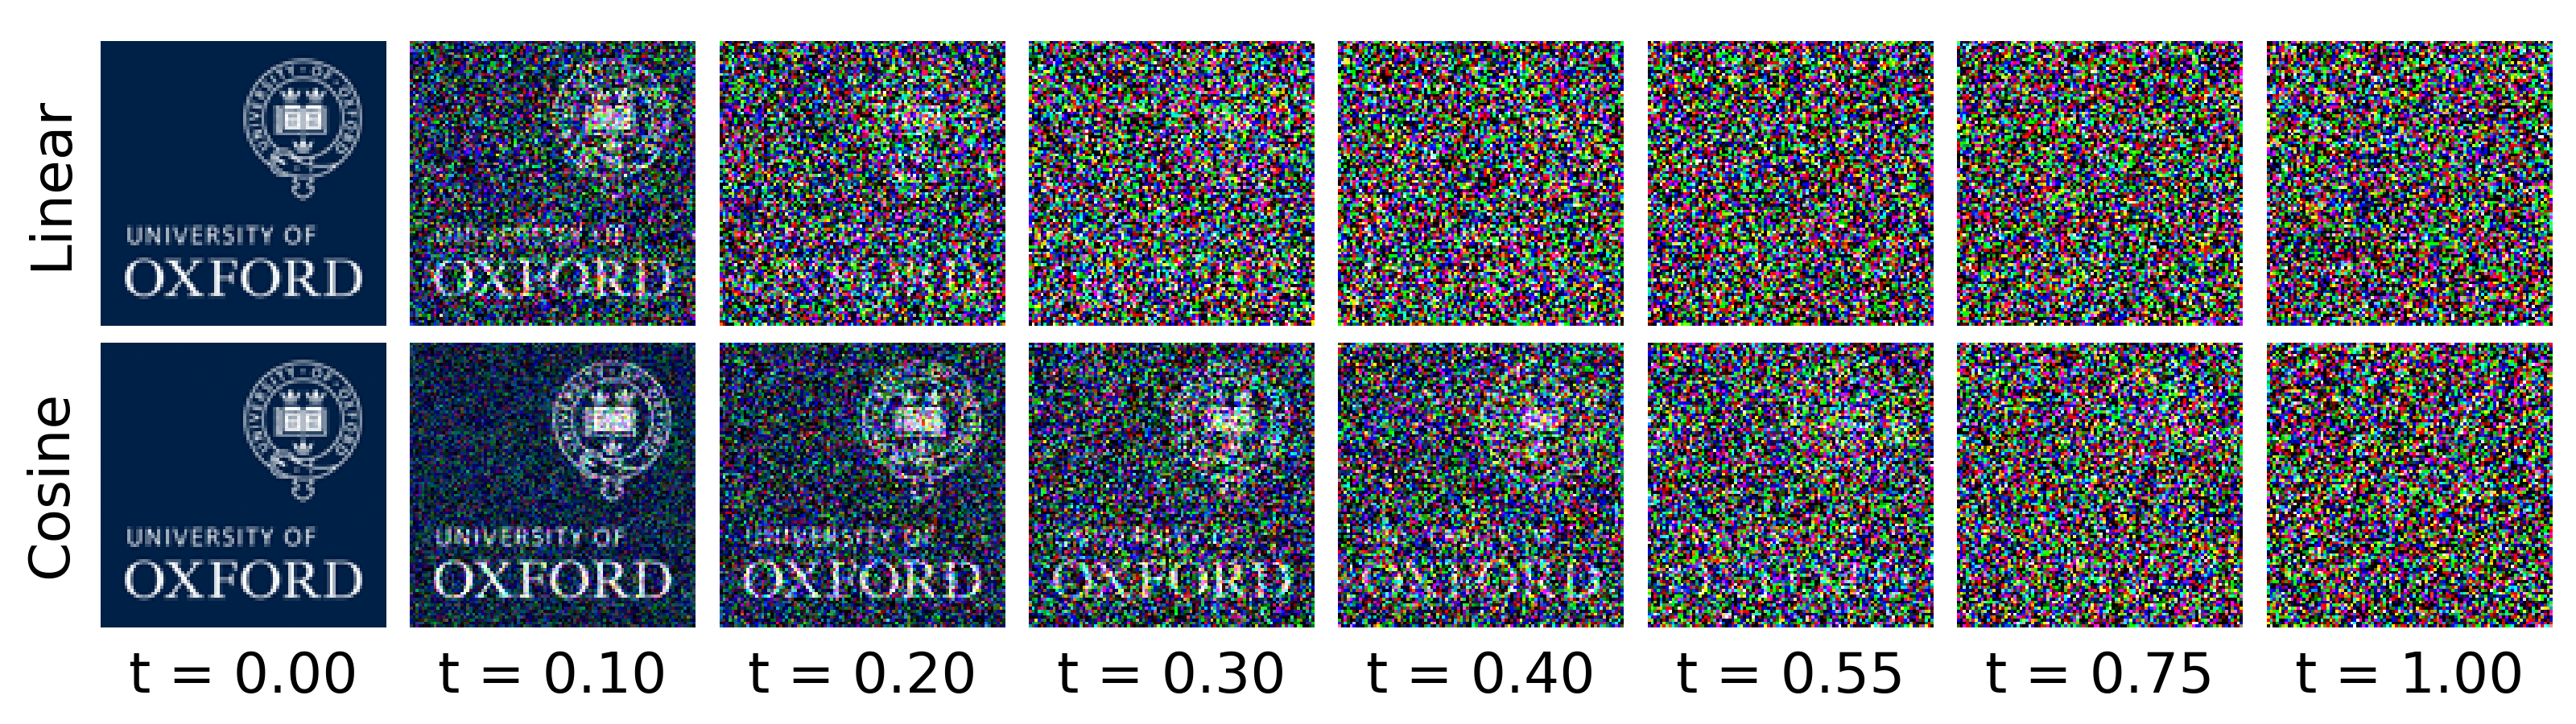
\includegraphics[width=\linewidth]{linear_vs_cosine.png}
    \caption{Linear schedule vs. cosine schedule.}
    \label{fig:schedule-linear-vs-cosine}
\end{figure}

Empirically, the cosine schedule improves sample quality and accelerates convergence compared to linear schedules. It balances the trade-off between injecting sufficient noise for diversity and preserving enough signal for stable training. Moreover, because it avoids excessively noisy late stages, fewer discretisation steps are needed during sampling, reducing computational cost.

In this dissertation, we adopt this cosine schedule as the forward diffusion process. This choice is motivated by its demonstrated effectiveness in image and structural generative tasks \citep{dhariwal2021DiffusionModelsBeat,saharia2022PhotorealisticTexttoImageDiffusion,watsonNovoDesignProtein2023}, and by its compatibility with the variance-preserving SDE formulation used in our score model, \cref{eq:cosine-beta}. All experiments in later chapters therefore use the cosine schedule as the default setting.

\subsection{Summary}
This chapter has established the theoretical foundations of score-based diffusion models, which form the core generative framework employed in this dissertation. We began by introducing the forward diffusion process, first in its discrete DDPM formulation and then in its continuous-time generalisation as a stochastic differential equation. We then derived the reverse-time SDE, showing that generative modelling reduces to the problem of score estimation. This led naturally to the denoising score matching objective, which enables training a neural network to approximate the score function across all noise levels. Finally, we discussed practical sampling algorithms, including reverse SDE integration and predictor-corrector methods, and examined the role of noise schedules, with particular emphasis on the cosine variance-preserving schedule adopted in this work.

Together, these elements provide a principled probabilistic framework for deep generative modelling. Unlike GANs or VAEs, score-based diffusion models avoid common issues such as mode collapse or restrictive latent assumptions, while offering strong theoretical guarantees and flexible sampling procedures. The remainder of this dissertation builds upon these foundations to adapt score-based diffusion to the setting of protein backbone generation, where structural constraints and geometric representations introduce unique modelling challenges.

\clearpage

\section{Protein Structure Modelling with Graph Neural Networks}\label{sec:protein-gnn}
\subsection{Proteins and Structural Constraints}\label{subsec:proteins-constraints}
Proteins are linear polymers of amino acids that fold into three-dimensional structures. Their backbone is a repeating chain of atoms N-C\(_\alpha\)-C, with side chains branching from C\(_\alpha\). In this work we adopt a C\(_\alpha\)-only representation: each residue \(i \in \{1,\dots,L\}\) is associated with a 3D coordinate \(x_i \in \mathbb{R}^3\). This representation is widely used for coarse-grained modelling because it captures the global geometry of the fold while keeping the state space compact.

Even at this coarse level, protein geometry is far from arbitrary. Neighbouring C\(_\alpha\) atoms exhibit a characteristic virtual bond length
\begin{align*}
    d_i \;=\; \|x_i - x_{i-1}\| \approx 3.8~\text{\AA},
\end{align*}
and local shape can be described by the virtual bond angle
\begin{align*}
    \theta_i \;=\; \angle(x_{i-1}, x_i, x_{i+1}),
\end{align*}
and the virtual dihedral
\begin{align*}
    \tau_i \;=\; \mathrm{dihedral}(x_{i-2}, x_{i-1}, x_i, x_{i+1}),
\end{align*}
whose empirical distributions are constrained by backbone sterics and peptide planarity. 
Beyond local geometry, valid structures avoid steric clashes (no two non-neighbour residues at unrealistically short distances) and typically exhibit compact, physically plausible folds. 

\paragraph{Scope of this work.}
Our goal is backbone-level generative modelling using score-based diffusion. We do not impose hard geometric constraints during training or sampling (e.g.\ fixed bond lengths/angles); instead, we learn the distribution over C\(_\alpha\) coordinate trajectories and evaluate fidelity against native backbones. Section~\ref{sec:Experiments} reports RMSD/TM results and discusses the limitation that high RMSD/low TM can still correspond to physically valid but non-native folds.

\paragraph{Paired evaluation vs.\ unconditional validity.}
Because each generated backbone is compared to its specific native target of the same length \(L\), RMSD/TM measure reconstruction fidelity, not absolute physical validity. 
This is appropriate for our benchmarking setting (paired evaluation), but one should interpret low TM or high RMSD with caution: a sample can be a plausible alternative fold while scoring poorly against the chosen native reference.

\subsection{Graph Representation of Backbones}\label{subsec:graph-repr}
% Nodes: residues (Cα coordinates); Edges: radius graph (and optional sequence edges);
% Edge features: radial basis of distances, unit direction, diffusion-time embedding; Node features: optional positional embedding (residue index).
A protein backbone of length \(L\) is represented as a graph \(G=(V,E)\), where each residue corresponds to a node and edges capture both geometric proximity and sequential connectivity. This formulation enables the use of graph neural networks as score models, allowing information to be propagated through local neighbourhoods while respecting the spatial structure of the backbone. 

\paragraph{Nodes.}
Each node \(i \in V\) corresponds to a residue with coordinate \(x_i \in \mathbb{R}^3\) representing the position of its C\(_\alpha\) atom. For simplicity, we do not include residue type or side-chain information in this work, focusing purely on the geometry of the backbone. The node features are initialised as positional embeddings derived from the residue index (Section~\ref{subsec:architectures}), along with optional time-conditioning features from the diffusion process.

\paragraph{Edges.}
Edges are constructed using a radius graph: for each node \(i\), we connect edges to all neighbours \(j\) within a cutoff distance \(r\), subject to a maximum of \(k\) nearest neighbours. Formally,
\begin{align*}
    (i,j) \in E \quad \Leftrightarrow \quad \|x_i - x_j\| \leq r \quad \text{and } j \text{ is among the } k \text{ closest to } i.
\end{align*}
This design ensures that local spatial relationships are captured without requiring a fixed sequence length. In addition to geometric edges, self-loops are included to stabilise message passing and allow each node to retain its own features. Edges are directed: for each \((i,j) \in E\), messages are passed from \(i\) (source) to \(j\) (target). This convention is consistent with the implementation of \texttt{TransformerConv} in PyTorch Geometric, and we do not duplicate edges to create an undirected graph.

\paragraph{Edge features.}
For each edge \((i,j) \in E\), we compute a feature vector combining geometric and diffusion-time information:
\begin{itemize}
    \item \textbf{Radial basis encoding:} The distance \(\|x_i - x_j\|\) is expanded into a vector using Gaussian radial basis functions,
        \begin{align*}
            \phi_\ell(\|x_i - x_j\|) = \exp\!\left(-\frac{(\|x_i - x_j\|-c_\ell)^2}{2\sigma^2}\right),
        \end{align*}
        for centres \(\{c_\ell\}_{\ell=1}^M\) distributed uniformly in \([0,r]\). This provides a smooth representation of distances. 
    \item \textbf{Directional encoding:} The normalised vector
        \begin{align*}
            d_{ij} = \frac{x_i - x_j}{\|x_i - x_j\|}
        \end{align*}
        encodes the relative orientation of the neighbour. This directional feature allows the network to capture local geometry beyond mere distances. 
    \item \textbf{Time embedding:} The diffusion timestep \(t\) is embedded into a high-dimensional feature \(e_t\) using sinusoidal positional encodings and projected through a linear layer. For each edge \((i,j)\), we associate \(e_t\) with the source node \(i\), enabling time-dependent conditioning of messages.
\end{itemize}
The full edge feature vector is then obtained by concatenation:
\begin{align*}
    h_{ij} = \big[ \; \text{radial basis} \;\|\; \text{direction} \;\|\; \text{time embedding} \;\big].
\end{align*}

\paragraph{Rationale.}
This graph construction has several desirable properties: (i) it is permutation-invariant to residue ordering, (ii) it scales linearly with the number of residues \(L\), (iii) it incorporates both distance and orientation information, which are critical for protein geometry, and (iv) it enables variable-length backbones to be handled naturally without padding. These features make it well-suited for score-based diffusion over protein structures.

\subsection{Score Models: Architectures}\label{subsec:architectures}
The score network \(s_\theta(x,t)\) is parameterised by a neural network that maps noisy protein backbones to score estimates. We explore several architectures of increasing complexity, culminating in a Transformer-based graph neural network that incorporates positional information.

\paragraph{Baseline: UNet on padded coordinates.}
As a baseline, we implemented a UNet architecture applied directly to backbone coordinates represented as sequences of fixed length. Each protein was zero-padded to a common maximum length, and the UNet operated on the resulting coordinate tensors. This design provides a simple convolutional benchmark but does not handle variable-length inputs naturally and discards explicit geometric relationships between residues. It serves primarily as a sanity check to compare graph-based approaches against a conventional deep learning model.

\paragraph{Baseline: TransformerConv without positional encodings.}
Our second baseline employs a graph neural network built from \texttt{TransformerConv} layers~\cite{PyG1.0,PyG2.0}, which extend graph attention mechanisms with edge features. 
The network consists of five stacked TransformerConv layers with residual connections and GraphNorm~\cite{cai2021GraphNormPrincipledApproach} normalisation. 
Edge features are given by the radial basis, directional vectors, and diffusion time embeddings described in Section~\ref{subsec:graph-repr}. 
This baseline captures geometric neighbourhood information but does not incorporate explicit positional encodings of residue indices, limiting its ability to represent sequential structure.

\paragraph{Main model: TransformerConv with positional encodings.}
Our main model extends the baseline TransformerConv GNN by incorporating sinusoidal positional embeddings of residue indices. 
For each node \(i\), we compute a positional encoding \(p_i \in \mathbb{R}^d\) using the standard formulation introduced for Transformers~\cite{vaswaniAttentionAllYou2017}, 
\begin{align*}
    p_{i,2k} = \sin\!\left(\frac{i}{10000^{2k/d}}\right), \quad p_{i,2k+1} = \cos\!\left(\frac{i}{10000^{2k/d}}\right),
\end{align*}
where \(d\) is the embedding dimension. These embeddings are projected through a linear layer and added to the initial node features, enabling the network to distinguish residues by their sequential position along the backbone.

\begin{remark} %TODO
    \textbf{Time Conditioning via Gaussian Fourier Features}
    Following \cite{song2021ScoreBasedGenerativeModeling}, we embed the diffusion time step \(t\in\left(0,1\right)\) using random Fourier features \cite{tancikFourierFeaturesLet2020}
    \begin{align*}
        \gamma\left(t\right)=\left[\cos\left(2\pi Wt\right),\sin\left(2\pi Wt\right)\right],\quad W\sim\mathcal{N}\left(0,s^2\right),
    \end{align*}
    to provide continuous and expressive encoding of time.
    \textbf{Positional Encoding for Node Order Awareness}
    Graph-based models are inherently invariant to node permutations, which can be a limitation when modeling protein backbones, where the sequential order of residues encodes biologically meaningful directionality along the chain. To inject this ordering information, each node is assigned a scalar index \(p\in\left[0,1\right]\) representing its normalized position in the sequence. This index is first mapped to a high-dimensional representation using a sinusoidal encoding \cite{vaswaniAttentionAllYou2017}
    \begin{align*}
        \rho\left(p\right)=\left[\sin\left(\omega_1 p\right),\cos\left(\omega_1 p\right),\sin\left(\omega_2 p\right),\cos\left(\omega_2 p\right),...\right]
    \end{align*}
    where \(w_k\)'s are fixed frequencies. The resulting positional embedding is then passed through a learnable transformation, such as a multilayer perceptron (MLP), before being incorporated into the model
\end{remark}

The model architecture is as follows:
\begin{itemize}
    \item \textbf{Input:} node features = positional embedding + time embedding; edge features = radial basis + direction + time embedding.  
    \item \textbf{Five TransformerConv layers:} each layer performs multi-head attention over neighbourhoods defined by the radius graph, using edge features to modulate attention weights. Residual connections are applied between layers.  
    \item \textbf{Normalisation:} GraphNorm is applied within each block to stabilise training.  
    \item \textbf{Output:} the network predicts the score vector \(s_\theta(x,t) \in \mathbb{R}^{3L}\), matching the dimensionality of the input coordinates.  
\end{itemize}

\paragraph{Residual structure.}
Residual connections are crucial in deep graph networks, particularly when stacking multiple attention layers. 
For each TransformerConv block, the output is added to the block input before normalisation:
\begin{align*}
    h^{(l+1)} = \mathrm{GraphNorm}\!\big(h^{(l)} + \mathrm{TransformerConv}(h^{(l)}, E)\big).
\end{align*}
This design improves gradient flow, stabilises optimisation, and enhances performance, particularly on long backbones.

\paragraph{Architectural choices.}
We experimented with both GraphNorm and LayerNorm as normalisation layers, finding GraphNorm to perform more consistently across models. 
BatchNorm was not suitable due to the highly variable protein lengths and small batch sizes. 
The choice of five TransformerConv layers reflects a balance between model expressivity and computational cost, given the memory requirements of neighbourhood-based attention. 

\paragraph{Summary.}
The UNet baseline provides a simple non-graph benchmark; the TransformerConv baseline demonstrates the benefit of neighbourhood-based attention without positional encodings; and the main TransformerConv model with positional embeddings forms the most expressive architecture, integrating geometric, sequential, and temporal information for score estimation.

\subsection{Training Setup}\label{subsec:training-setup}
% Loss (denoising score matching), cosine VP schedule (simplified cosine form), sampler (predictor–corrector), data processing (CATH S40, CA extraction), hyperparameters.
Having defined the representation and model architectures, we now describe the training setup used to learn score networks for protein backbone generation.

\paragraph{Dataset.}
We train and evaluate on the CATH S40 dataset, a widely used benchmark for structural modelling tasks. 
This dataset clusters protein domains at \(40\%\) sequence identity, ensuring reduced redundancy while maintaining structural diversity. 
For each structure, we extract the backbone coordinates by retaining only the C\(_\alpha\) atom of each residue. 
Backbones are represented as variable-length sequences of C\(_\alpha\) coordinates \(\{x_i \in \mathbb{R}^3\}_{i=1}^L\), which are then converted into graphs as described in Section~\ref{subsec:graph-repr}. 
We split the dataset into training, validation, and test sets at the domain level to avoid leakage between structurally similar proteins.

\paragraph{Forward process and noise schedule.}
We adopt the variance-preserving (VP) SDE formulation with the cosine noise schedule introduced by \cite{nicholImprovedDenoisingDiffusion2021}. Specifically, the cumulative noise attenuation is defined as
\begin{align*}
    \bar \alpha_t = \cos^2\!\left(\frac{t+s}{1+s}\cdot \frac{\pi}{2}\right),
\end{align*}
with a small offset \(s = 10^{-4}\) to avoid singularities. Unlike the normalised version, we omit the denominator, which means that \(\bar\alpha_0 < 1\) and the process injects negligible noise even at \(t=0\). This simplified form has been adopted in prior implementations and provides a stable and effective noise schedule in practice. 

\paragraph{Loss function.}
Training follows the denoising score matching objective described in Section~\ref{sec:SBD}. For a random timestep \(t \sim \mathcal{U}(0,1)\), we sample noisy coordinates
\begin{align*}
    x_t = \sqrt{\bar\alpha_t}\,x_0 + \sqrt{1-\bar\alpha_t}\,\epsilon, \quad \epsilon \sim \mathcal{N}(0,I),
\end{align*}
and minimise the mean squared error between the predicted noise \(\epsilon_\theta(x_t, t)\) and the true noise \(\epsilon\). 
Equivalently, this trains \(s_\theta\) to approximate the score \(\nabla_x \log p_t(x)\) up to a known scaling factor.

\paragraph{Sampling.}
At test time, new structures are generated by simulating the reverse SDE using predictor-corrector sampling \cite{song2021ScoreBasedGenerativeModeling}. 
Starting from Gaussian noise \(x_T \sim \mathcal{N}(0,I)\), the process alternates between predictor steps (Euler-Maruyama updates of the reverse SDE) and corrector steps (Langevin dynamics refinements). 
This yields improved fidelity compared to predictor-only integration.

\paragraph{Optimisation.}
Models are trained using the Adam optimiser (Kingma and Ba, *ICLR 2015*) with a learning rate of \(10^{-4}\) and weight decay of \(10^{-6}\). We use a batch size adapted to GPU memory constraints (typically between 16 and 32 backbones, depending on length). Mixed-precision training is employed to reduce memory usage. Training proceeds for \(300\) epochs with early stopping based on validation loss. 

\paragraph{Implementation.}
All models are implemented in PyTorch and PyTorch Geometric \citep{PyG1.0,PyG2.0}. Radius graphs are constructed on-the-fly at each forward pass using efficient neighbour search. Training and evaluation were performed on NVIDIA GPUs with \(48\)GB of memory.

\subsection{Summary}\label{subsec:method-summary}
In this section we described the methodology for adapting score-based diffusion models to the task of protein backbone generation. We began by outlining the structural constraints of proteins and motivated the use of a C\(_\alpha\)-only representation. We then formulated backbones as graphs, with nodes corresponding to residues and edges defined through a radius neighbourhood, augmented by radial basis encodings, directional features, and diffusion-time embeddings. This representation allows geometric information to be captured in a permutation-invariant manner while naturally supporting variable-length backbones.

We explored three architectures for the score network: a UNet baseline on padded coordinate sequences, a TransformerConv-based graph neural network without positional encodings, and our main model, a residual TransformerConv GNN with positional embeddings. The latter integrates geometric, sequential, and temporal information and demonstrated the strongest expressive capacity in preliminary tests. Architectural design choices, including residual connections and GraphNorm, were discussed in detail.

Finally, we presented the training setup, including the variance-preserving SDE with a cosine noise schedule, the denoising score matching loss, predictor-corrector sampling, and optimisation procedures. Together, these elements define a principled and practical framework for learning score-based diffusion models on protein backbones.

The next section reports experimental results, benchmarking these models on the CATH S40 dataset using both quantitative metrics (RMSD, TM-score) and qualitative visualisations.

\clearpage

\section{Experiments}\label{sec:Experiments}
This section presents the experimental evaluation of the score-based diffusion models described in Section~\ref{sec:protein-gnn}. We benchmark three architectures on the CATH S40 dataset and assess their performance using quantitative metrics and qualitative visualisations. 

\subsection{Dataset and Preprocessing}\label{subsec:dataset}
% --- To fill in ---
% - Mention CATH S40 split sizes (train / validation / test).
% - Any filtering or preprocessing steps.
% - Statistics (e.g., distribution of backbone lengths).
% (Optionally include a table or histogram figure here.)

\subsection{Evaluation Metrics}\label{subsec:metrics}
We evaluate reconstruction fidelity using two standard structural similarity measures:
\begin{itemize}
    \item \textbf{Root-mean-square deviation (RMSD):}
        \begin{align*}
            \mathrm{RMSD}(X, Y) = \sqrt{\frac{1}{L}\sum_{i=1}^{L} \|x_i - y_i\|^2},
        \end{align*}
        where \(X=\{x_i\}\) and \(Y=\{y_i\}\) are two aligned backbones of length \(L\). Lower RMSD indicates closer correspondence to the reference.
    \item \textbf{TM-score:} a length-normalised measure of structural similarity ranging from \(0\) to \(1\), with higher values indicating better alignment. Unlike RMSD, TM-score is less sensitive to local errors and more reflective of global fold similarity.
\end{itemize}

We also report the raw training error (MSE between predicted and true noise) as an auxiliary metric.

\subsection{Quantitative Results}\label{subsec:results}
% --- To fill in ---
% Insert a main comparison table here:
% Model | RMSD (mean ± std) | TM-score (mean ± std) | Error
% - TransformerConv + PosEnc (main)
% - TransformerConv w/o PosEnc (baseline)
% - UNet (baseline)
% You may also add per-length results if relevant.

\begin{table}[htbp]
\centering
\caption{Quantitative performance on the CATH S40 test set. Values are mean ± standard deviation across structures.}
\label{tab:results}
\begin{tabular}{lccc}
\hline
Model & RMSD (\(\downarrow\)) & TM-score (\(\uparrow\)) & Error (\(\downarrow\)) \\
\hline
TransformerConv + PosEnc (ours) &   &   &   \\
TransformerConv (no PosEnc)     &   &   &   \\
UNet (padded)                   &   &   &   \\
\hline
\end{tabular}
\end{table}

\paragraph{Distribution analysis.}
In addition to summary statistics, we plot the distribution of RMSD and TM-scores across the dataset (Figure~\ref{fig:rmsd-hist} and Figure~\ref{fig:tm-hist}). 
These histograms reveal the variability of model performance across different protein domains.

\begin{figure}[htbp]
\centering
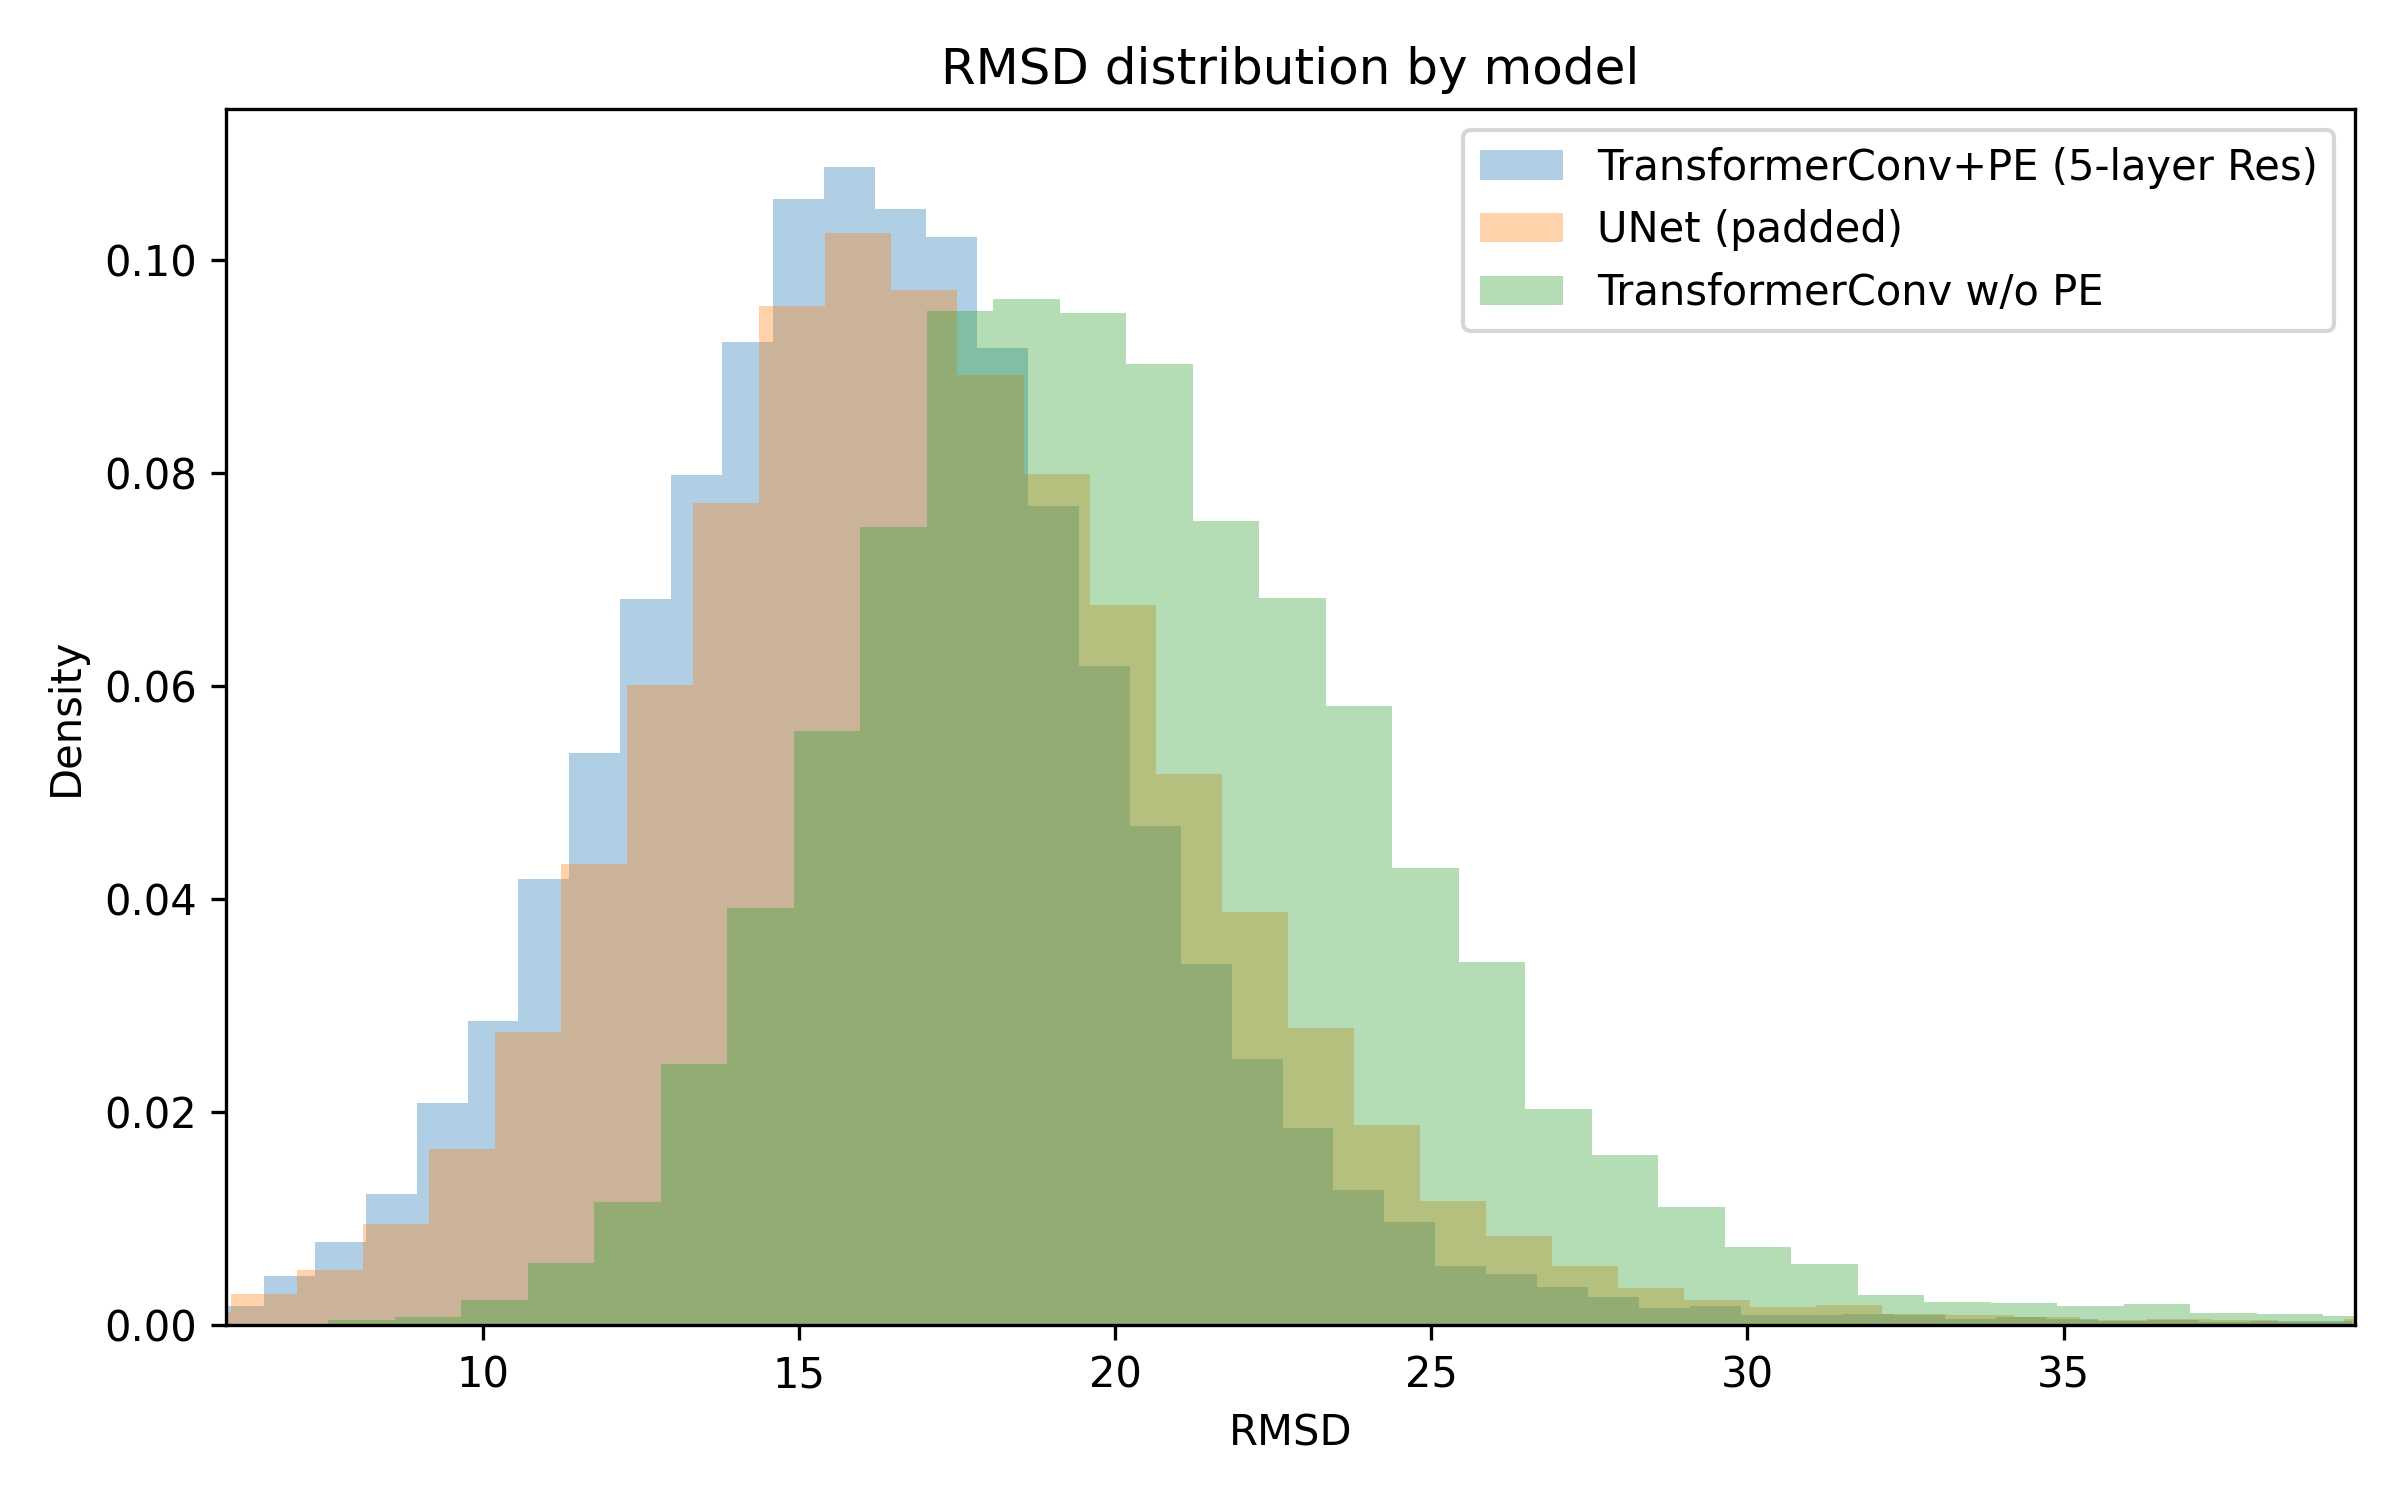
\includegraphics[width=0.7\linewidth]{rmsd_dist.png}
\caption{Distribution of RMSD values across test structures. Lower is better.}
\label{fig:rmsd-hist}
\end{figure}

\begin{figure}[htbp]
\centering
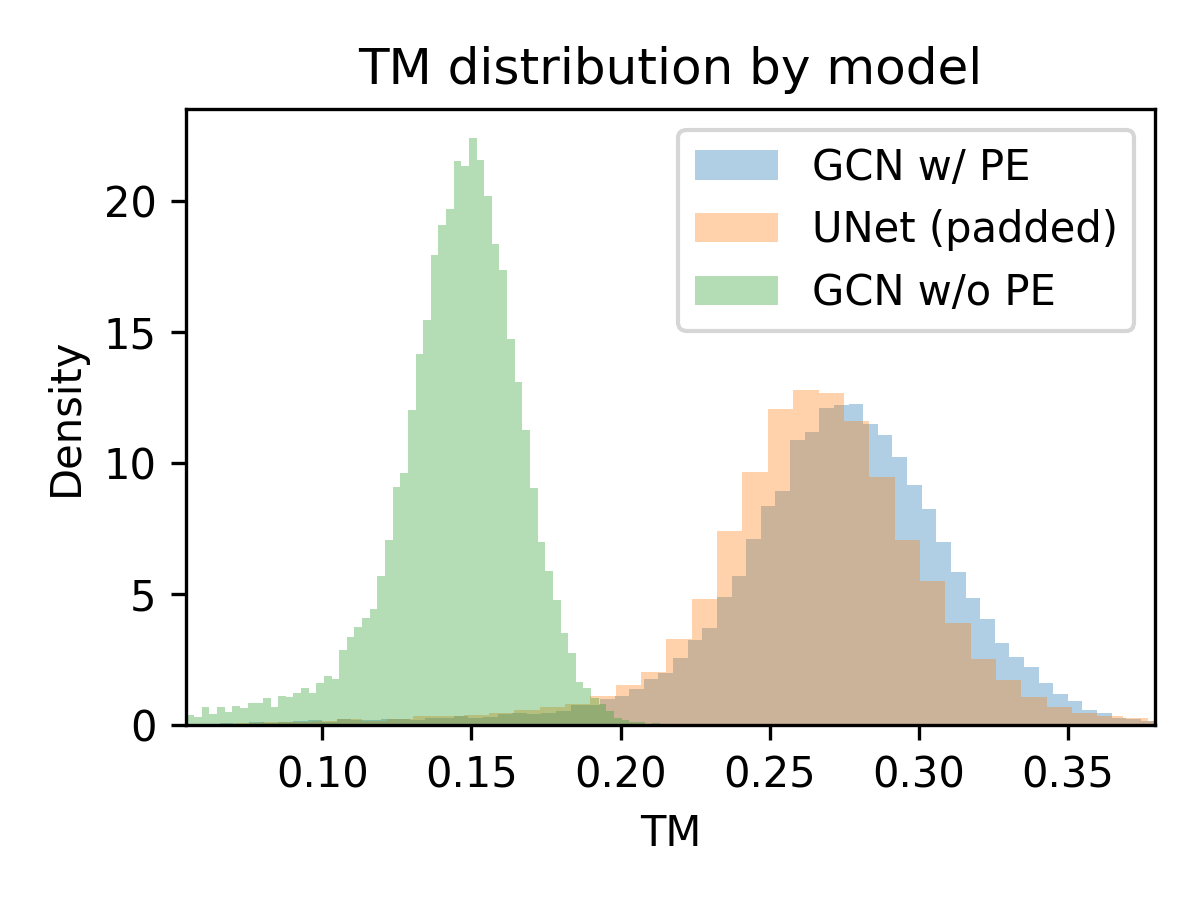
\includegraphics[width=0.7\linewidth]{tm_dist.png}
\caption{Distribution of TM-scores across test structures. Higher is better.}
\label{fig:tm-hist}
\end{figure}

\paragraph{Scatter plots.}
We further analyse performance as a function of backbone length \(L\), plotting RMSD and TM-score versus \(L\) (Figure~\ref{fig:rmsd-vs-l}, Figure~\ref{fig:tm-vs-l}).

\begin{figure}[htbp]
\centering
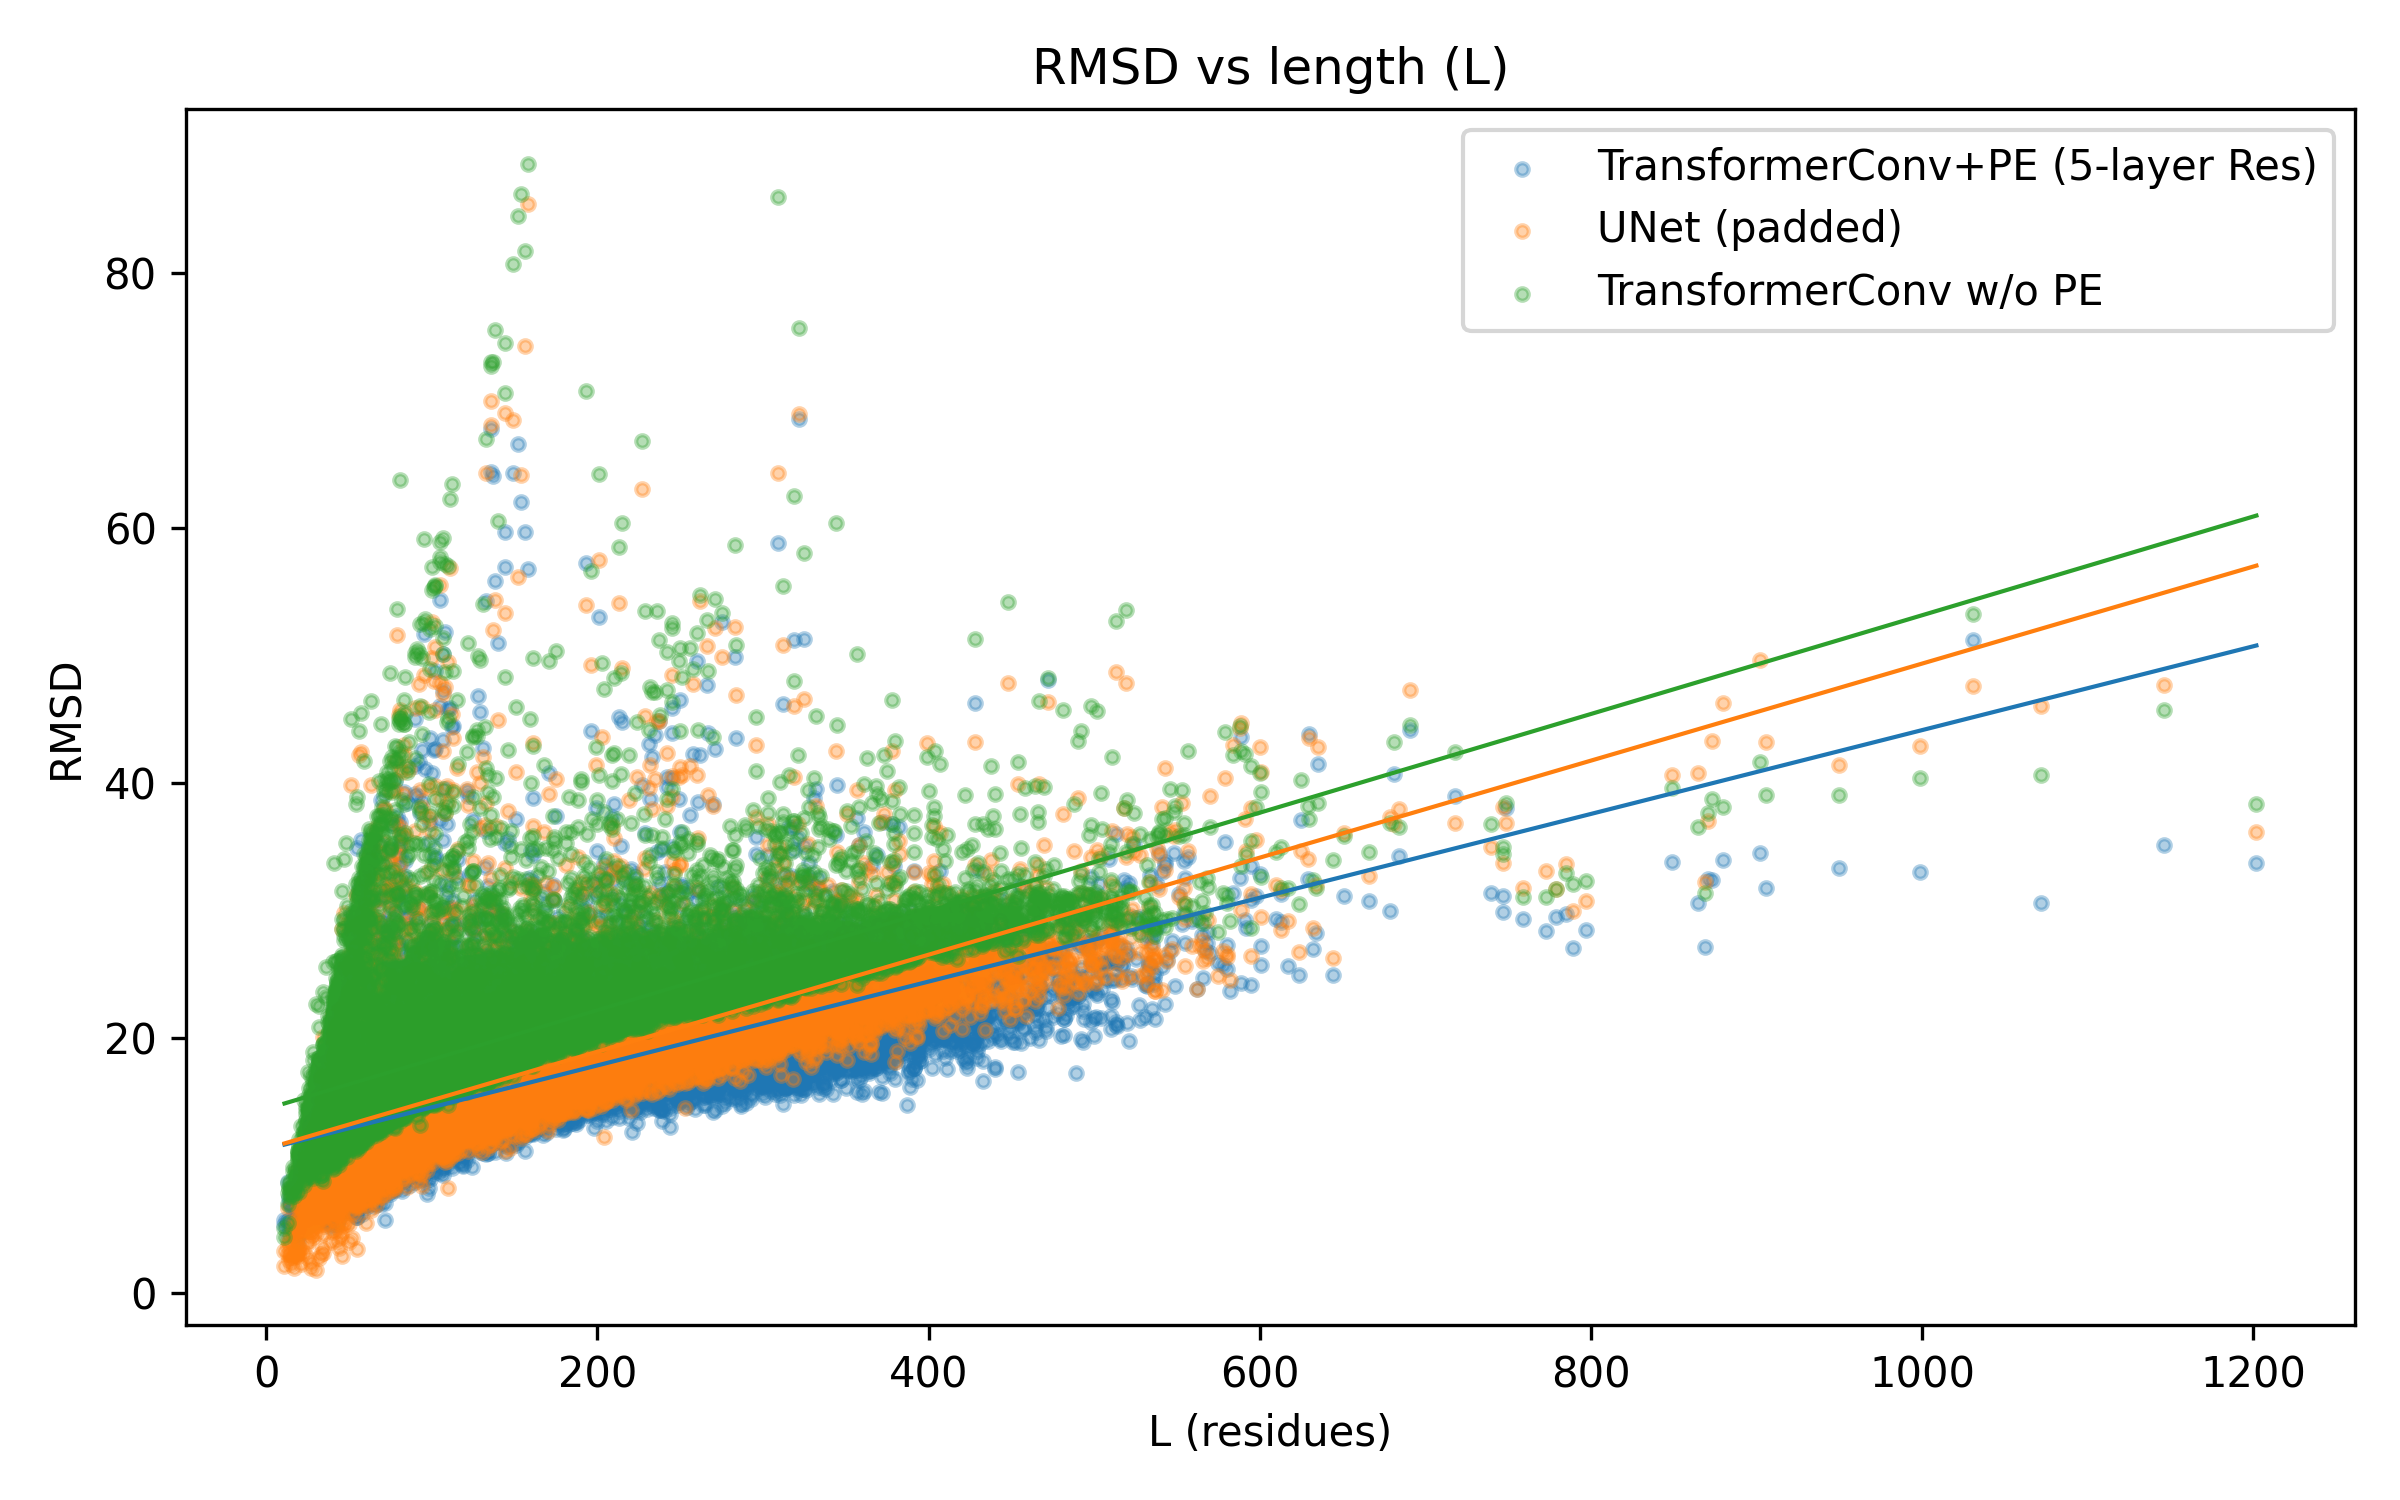
\includegraphics[width=0.7\linewidth]{rmsd_vs_L.png}
\caption{RMSD versus backbone length.}
\label{fig:rmsd-vs-l}
\end{figure}

\begin{figure}[htbp]
\centering
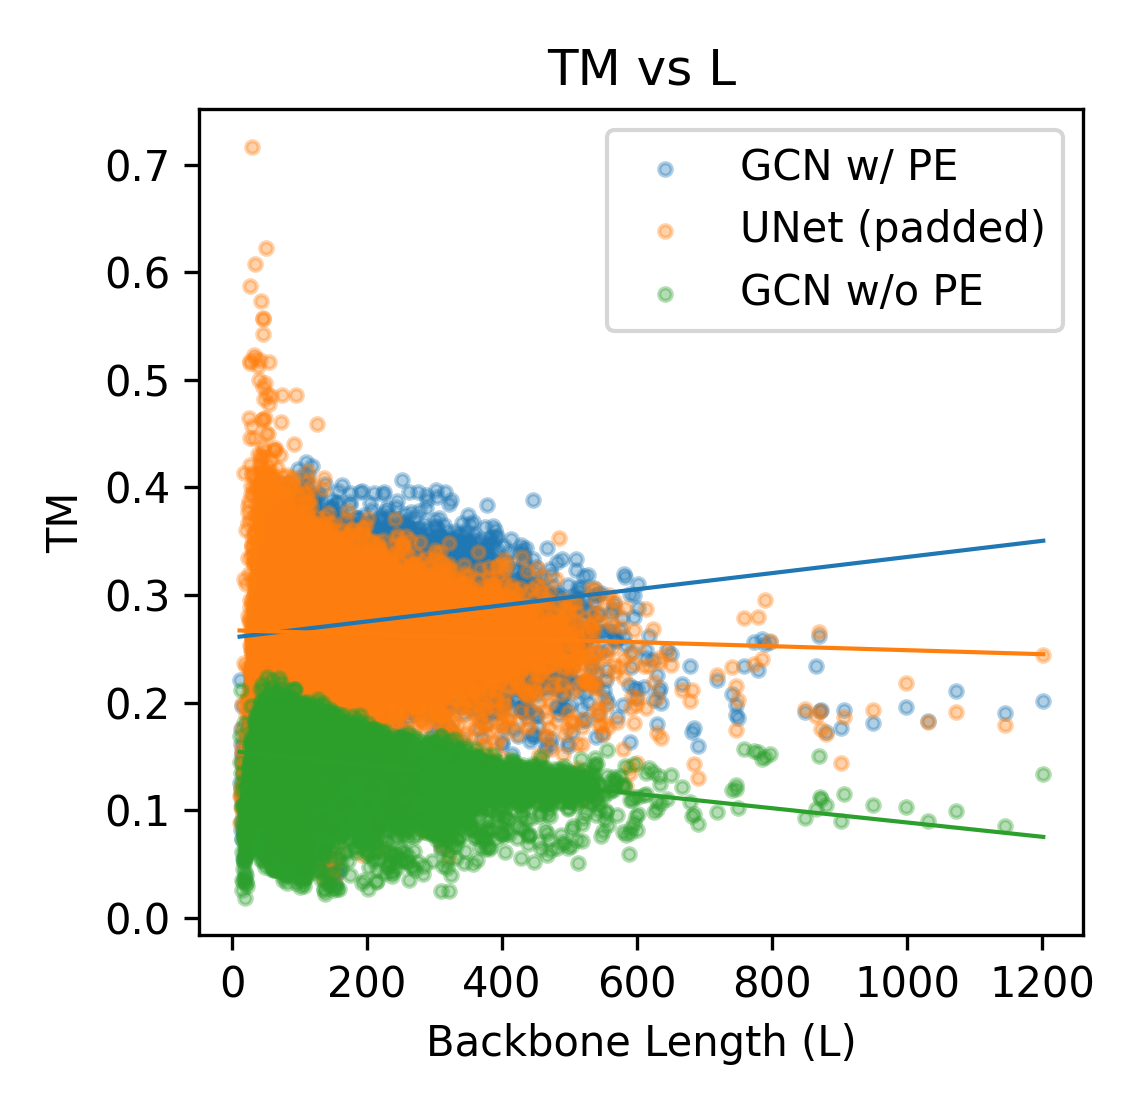
\includegraphics[width=0.7\linewidth]{tm_vs_L.png}
\caption{TM-score versus backbone length.}
\label{fig:tm-vs-l}
\end{figure}

\subsection{Ablation Studies}
\label{subsec:ablations}

To isolate the effect of architectural components, we conducted ablations:
\begin{itemize}
    \item \textbf{Positional encodings:} comparing TransformerConv with and without positional embeddings.
    \item \textbf{Normalisation:} GraphNorm versus LayerNorm.
\end{itemize}

% --- Insert small comparison table or plots here. ---

\subsection{Qualitative Visualisation}\label{subsec:visualisation}
Finally, we present visualisations of generated backbones using PyMOL. For each test structure, we overlay the generated backbone with the native structure (Figure~\ref{fig:pymol-example}), highlighting both successes (low RMSD/high TM) and failures (plausible but non-native folds).

\begin{figure}[htbp]
    \centering
    % \includegraphics[width=0.6\linewidth]{pymol_example.png}
    \includegraphics[width=0.6\linewidth]{example-image}
    \caption{Example PyMOL visualisation of generated backbone (blue) aligned with native structure (grey).}
    \label{fig:pymol-example}
\end{figure}

\subsection{Summary of Results}\label{subsec:results-summary}
% --- To write after results are in ---
% - Briefly summarise the key findings (ours > baselines, importance of positional encodings, etc.).
% - Transition to Chapter 5.

\clearpage

\section{Discussion and Conclusion}\label{sec:Discussion_and_Conclusion}
\subsection{Discussion of Results}\label{subsec:discussion-results}
The experiments in Section~\ref{sec:Experiments} demonstrate that score-based diffusion models can generate protein backbones with meaningful structural similarity to native folds. Our main model, the TransformerConv GNN with positional embeddings, consistently outperformed the baselines in both RMSD and TM-score. This highlights the importance of incorporating sequential information into graph-based architectures, in addition to geometric edge features. 

The ablation studies further show that GraphNorm provided more stable training than LayerNorm, particularly for variable-length proteins. Meanwhile, the UNet baseline performed poorly, underscoring the limitations of sequence-padded architectures that ignore protein geometry. 

\subsection{Limitations}\label{subsec:limitations}
While results are encouraging, several limitations must be acknowledged:
\begin{itemize}
    \item \textbf{Evaluation metrics.} RMSD and TM-score measure similarity to a specific native fold of length \(L\). However, a generated backbone with high RMSD or low TM may still correspond to a physically plausible alternative fold. Thus, our evaluation measures reconstruction fidelity rather than unconditional validity.
    \item \textbf{Backbone-only representation.} We model only C\(_\alpha\) atoms, ignoring side chains and residue types. This limits biological interpretability and applicability to sequence-conditioned design.
    \item \textbf{Geometric constraints.} We did not enforce hard bond length or bond angle constraints during training or sampling. Although the model learns approximate geometry from data, explicit constraints would ensure chemical validity.
    \item \textbf{Model scale.} Our models are relatively small compared to state-of-the-art generative protein models. Larger networks with equivariant layers or global attention may further improve results.
\end{itemize}

\subsection{Future Work}\label{subsec:future-work}
Several promising directions follow from this study:
\begin{itemize}
    \item \textbf{Constraint integration.} Future models could enforce bond lengths, bond angles, and chirality constraints explicitly within the diffusion dynamics.
    \item \textbf{Sequence conditioning.} Extending the framework to sequence-to-structure generation would enable protein design tasks directly relevant to biology and drug discovery.
    \item \textbf{Advanced architectures.} Incorporating SE(3)-equivariant GNNs, Graph GPS layers, or global attention could capture long-range dependencies more effectively.
    \item \textbf{Evaluation metrics.} Beyond RMSD and TM-score, metrics that capture physical validity or functional plausibility would provide a more nuanced evaluation of generated backbones.
\end{itemize}

\subsection{Conclusion}\label{subsec:conclusion}
This dissertation has presented an adaptation of score-based diffusion models to the task of protein backbone generation. We derived the theoretical foundations of score-based diffusion, constructed graph-based representations of protein structures, and developed several neural architectures for score estimation. Through experiments on the CATH S40 dataset, we demonstrated that a residual TransformerConv GNN with positional embeddings achieves improved performance over both non-graph and graph baselines. 

Overall, this work illustrates the potential of diffusion generative models for structural biology and provides a foundation for future research in protein design. By integrating probabilistic rigour with graph-based learning, score-based diffusion offers a principled and flexible framework for exploring the immense space of protein structures.

\clearpage

\section*{Appendix}
\begin{verbatim}
Put your R code here.
\end{verbatim}

\clearpage

\bibliographystyle{apalike}
\bibliography{references}
\end{document}
